\documentclass[8pt,titlepage]{article}
\usepackage[utf8]{inputenc} 
\usepackage[english]{babel}
\usepackage{tikz}
\usepackage{fancyvrb}
\usepackage{tikz}

\title{EDA040 Camera Project [Axis \& Androids]} 
\begin{Large}
\author{Jakob Grundström, pi07jg8 \\Bengt Ericsson, dt08be9 \\Carl Bjerggaard (vv06cb3) \\Magnus Törnqvist, dt08mtX}
\end{Large}

\begin{document}
\maketitle

\section{System Design}

\subsection{Overview}
A client has for each connected camera:
\begin{itemize}
\item SendThread
\item ReceiveThread
\item DisplayThread
\end{itemize}

and a camera server has for a client corresponding
\begin{itemize}
\item SendThread
\item ReceiveThread
\end{itemize}

\noindent Together these threads make up the basis of the image transferring and messaging of this system. Furthermore, the system consists on the server side of a

\begin{itemize}
\item CameraThread
\item CameraMonitor
\end{itemize}

and on the client side of
\begin{itemize}
\item DisplayMonitor
\item GUI classes
\end{itemize}

These will be described in more detail in the following sections.

\subsection{Networking}
The networking between a client and a server is handled by a SendThread and a ReceiveThread on each end. Both thread classes make use of a common Connection object, holding a socket, and providing high level networking. By design the sending and receiving should be concurrent.


\subsubsection{ReceiveThread}
A ReceiveThread typically waits in its run-loop until it gets a command integer, according to the protocol described below, and then chooses an appropriate action. The actions on the client side are, handled by ClientReceiveThread:
\begin{itemize}
\item handleImage() - which receives a byte array containing an image an puts it in a corresponding DisplayThreads FrameBuffer mailbox.
\item handleDisplayMode() - changing the display mode on request from the camera server. This method is called when a camera server detects motion and display mode should be switch to MOVIE. The display mode is then propagated to all other connected camera servers via the subscribed SendThread mailboxes in the DisplayMonitor.
\end{itemize}

The ServerReceiveThread only needs to handle display mode switching on request from the client’s end. Both the client’s and the servers ReceiveThreads are subclasses of ReceiveThreadSkeleton.

\subsubsection{SendThread}
A SendThread is a cyclic thread which waits for commands and/or images to be put in its or one of its mailboxes. Upon a receive on a mailbox the command or image is dispatched to its proper location. 

The ServerSendThread receives commands to its CircularBuffer mailbox fetched with a non-blocking tryGet() method and images to its FrameBuffer mailbox. These are then dispatched to the client via the SendThreads Connection object.

The ClientSendThread gets commands posted to its CircularBuffer mailbox. The commands can be from the GUI or from ClientReceiveThread which propaget display mode changes when received.

\subsubsection{Network protocol}
The network protocol will consist of messages being sent by a Connection object. Each message is initialized with a command integer. The system make use of two different message types as given by the table below.

%\begin{table}[h!]
%    \begin{tabular}{|l|l|}
%    	\caption{The network protocol used for sending command integers and mode flags.}
%    	\label{tableprot}
%        \hline
%        \textbf{Command} & \textbf{Format} \\ \hline
%        Image   & \begin{tabular}{l|l|l}
%        
%        Command & Length & Byte Array \\
%        
%    \end{tabular}
%     \\ \hline
%        Mode    & \begin{tabular}{l|ll}
%       
%        Command & Mode~~ & ~~~~~~~~~~~~~~\ \\
%        
%    \end{tabular}     \\
%        \hline
%    \end{tabular}
%\end{table}

\begin{figure}[hbp]
\centering
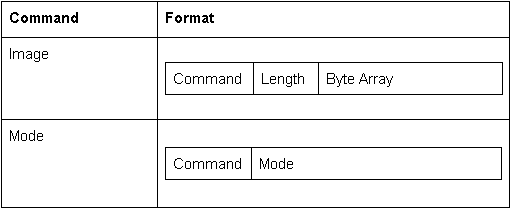
\includegraphics[width=0.75\textwidth]{../screenshots/tabell.png}
\caption{The network protocol used for sending command integers and mode flags.}
\end{figure}


\noindent The command integers and mode flags are defined in the class Protocol.


\section{Client side}

\subsection{DisplayThread}
Upon receiving an image frame the ReceiveThread puts it in its corresponding DisplayThread’s FrameBuffer mailbox. The DisplayThread’s taks is then to synchronized with other DisplayThreads display this image through methods provided by the GUI.

When the display mode is set to SYNC several DisplayThreads synchronize through their shared DisplayMonitor and the synchronized method syncFrames(). To determine if the delay difference if larger than a display difference threshold, which would implicate it is time to switch to mode AUTO, another monitor method is called from inside syncFrames(), it is called chooseSyncMode() and can change the synchronization mode.

When the display mode is set to ASYNC each DisplayThread instead call a local method called
asyncAsFastAsPossible(). This method as the name suggests render the images as soon as the are fetched from the FrameBuffer.

When the mode is set to AUTO each DisplayThread like in ASYNC mode calls asyncAsFastAsPossible() but in addition a DiplayMonitor method chooseSyncMode() to automatically determine if the delay difference between two DisplayThread images is smaller than a certain delay difference threshold. If so, the mode is switched to SYNC.

\subsubsection{DisplayMonitor with synchronized and asynchronized image viewing}
Each display in the configuration is provided image frames by a DisplayThread containing a FrameBuffer mailbox. The DisplayThreads are synchronized through a common DisplayMonitor.

\begin{itemize}
\item \textbf{Synchronous Mode} DisplayThreads put the (timestamp, id) of the next frame of the buffer in the DisplayMonitor’s priority queue. Then a DisplayThread has to wait until the time according to the timestamp is correct and until it is the first image in the priority queue. When the conditions are fulfilled the delay between creation time and show time is calculated and the sync mode is determined. Then after the DisplayThread leaves the monitor it is permitted to show its frame. 	
\item \textbf{Asynchronous Mode} DisplayThreads are permitted to independently show their image frames as fast as possible.
\item \textbf{Auto Mode} DisplayThreads are permitted to independently show their image frames as fast as possible though the delays are calculated and show time is calculated and the sync mode is determined. If the difference between delays is low the sync mode is changed to synchronous.
\end{itemize}

If the client receives images more than 0.2 seconds apart it should automatically enter Auto mode with asynchronous rendering; otherwise it should stay in synchronous mode. If the client is put in Async mode it stays in that mode.

\subsubsection{SyncFrames}
\begin{verbatim}
private long lag = TARGET_DELAY;
public synchronized long syncFrames(long timestamp) throws InterruptedException {
		timestamps.offer(timestamp);

		/* Calculate showtime for this thread in relation to FIRST SHOWN FRAME. */
		long showtime_new = lag + timestamp;				
		long diffTime;	// Time to showtime_new

		/* Wait until it is:
		 * 1) The right time.
		 * 2) timestamp less than all other timestamps.				*/				
		while ((diffTime = showtime_new - System.currentTimeMillis()) > 0) {
			Thread.sleep(diffTime);		
		} 

		while (timestamp > timestamps.peek()) { // Maybe check timestamp difference too, hmmm
			wait();
		}

		/* SHOW TIME */
		timestamps.remove();
		notifyAll();

		/* Calculate and return delay */
		long delay = System.currentTimeMillis() - timestamp;					
		chooseSyncMode(Thread.currentThread().getId(), delay);
		return delay; // The real delay
	}


\end{verbatim}
\subsubsection{chooseSyncMode}
\begin{verbatim}
long id_last = 0;
long delay_last = 0;	

public synchronized int chooseSyncMode(long id, long delay) {	// RESOLVE !!!		
		if (sync_mode == Protocol.SYNC_MODE.AUTO || sync_mode == Protocol.SYNC_MODE.SYNC) {
			if (id != id_last) {
				long dist = Math.abs(delay_last - delay);
				if (dist >= DELAY_SYNCMODE_THRESHOLD_MS) {
					sync_mode = Protocol.SYNC_MODE.AUTO;
				} else {
					sync_mode = Protocol.SYNC_MODE.SYNC;
				}
				id_last = Thread.currentThread().getId();
				delay_last = delay;		
			}
		}
		return sync_mode;
	}
}	
\end{verbatim}

\subsection{Desktop version}
The desktop part of our surveillance solution consist of a minimalistic client application written with Swing. The client is started from the command line with the camera server hosts and ports as arguments. The client support viewing of more than two connected cameras but of course the performance will degrade when more cameras are connected. Even though the synchronization is designed with several concurrent displays in mind the automatic synchronization mode switching is not, but it can still do the job if the delay differences small enough.

\begin{figure}[hbp]
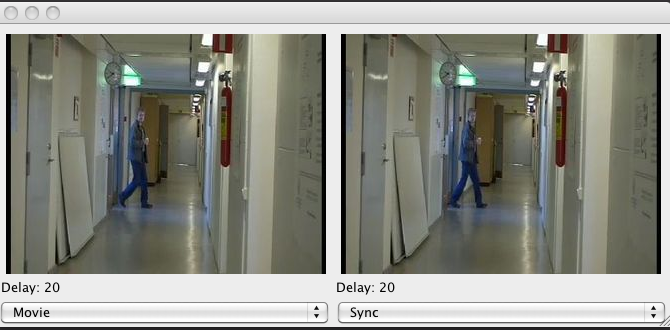
\includegraphics[width=0.75\textwidth]{../screenshots/desktopclient.png}
\caption{Screenshot of desktop client}
\label{desktopclient}
\end{figure}

When stared the Desktop Client Application is easy to use. The display mode is shown and set with the drop down menu to the left and the synchronization mode by the drop down menu to the right. The current delay for each image is shown under the images respectively.

Below is an UML diagram over the Desktop Client system. 

As one can tell from the UML diagram, the DesktopClient consists of three basic parts. The GUI, a send thread and a recieve thread. A simple but effective design.

\clearpage
\begin{figure}[h!]
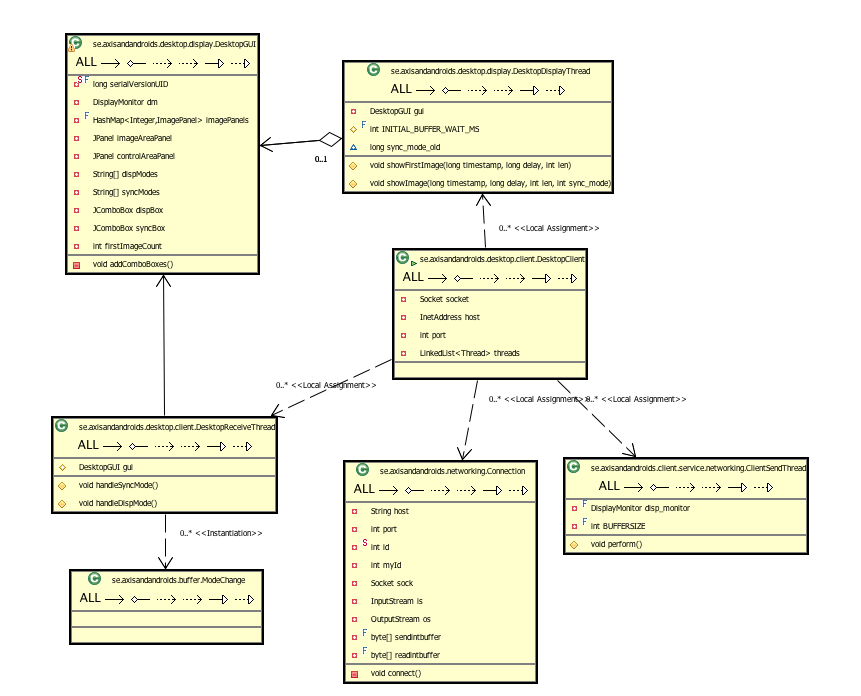
\includegraphics[width=2.0\textwidth]{../uml/desktop-client.png}
\caption{UML of the desktop client}
\end{figure}

\clearpage

\subsection{Android version}
The android version was created to have a portable surveillance station.

The difference between a desktop client based on Swing and a client built with the Android SDK is a matter of two different paradigms and frameworks. Swing has a long track record for being used as a framework to build heavy desktop clients, while Android is a new operating system for mobile devices. 

While developing the mobile client for our real-time concurrent surveillance application there were some difficulties apparent in the amount of new skills required to produce optimal results. 

Several obstacles appeared during the different phases of production - socket programming between the mobile client device and server, how to achieve a decent user interface and an equally appropriate user experience meanwhile maintaining the required concurrency and real-time constraints. 

Android is different from Swing, it uses a hierarchy based structure (with MVC, Model-View-Controller) that promotes modular programming and feels very intuitive to the programmer. The documentation provided by the Android SDK team is almost entirely flawless, albeit the unfamiliar tools and inexperience with mobile development as well as the new approach to programming in Android was the result of most obstacles that we caused ourselves.
Intents are used for different types of user interaction, activities are subparts of intents and Views are used to render the different activities. 

Screenshots from the Android application in action, running on the Android Virtual Machine, is shown below. First the user is presented with a connect view. After connection information is entered the user gets into display mode by pressing menu and then choosing display. Then then the display view is entered.

\begin{figure}[hbp]
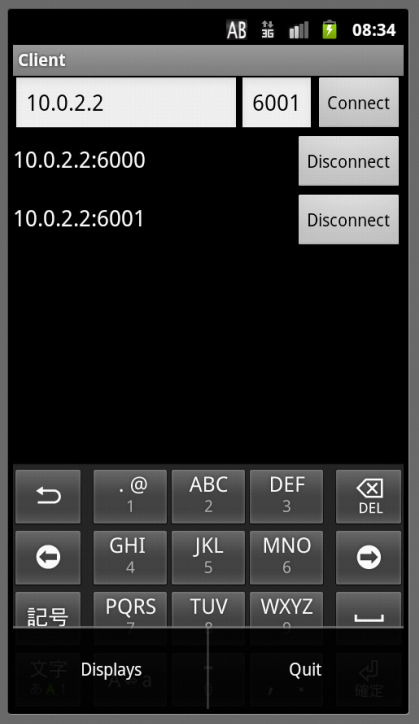
\includegraphics[width=0.75\textwidth]{../screenshots/androidConnecting.png}
\caption{Screenshot of the Android client connection menue}
\end{figure}


\begin{figure}[hbp]
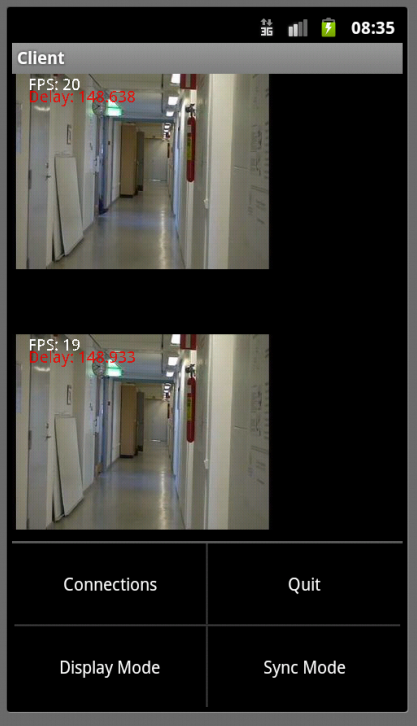
\includegraphics[width=0.75\textwidth]{../screenshots/androidDisplaying.png}
\caption{Screenshot of the Android client displaying the fakecamera}
\end{figure}

From the menu in display view the user can select Display Mode and Sync Mode. Modes are set as in the following screen shots.

\begin{figure}[hbp]
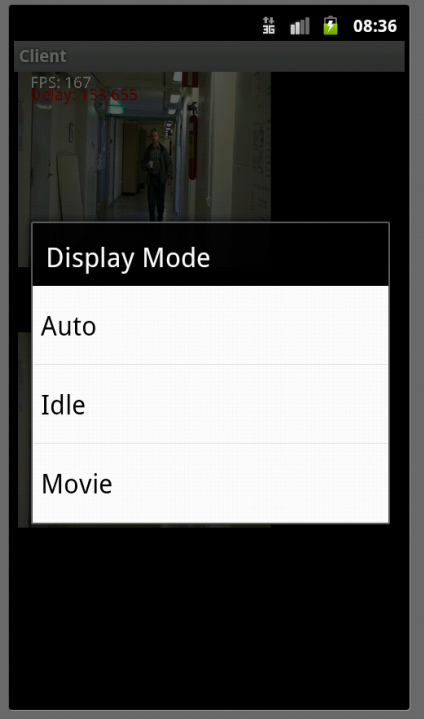
\includegraphics[width=0.75\textwidth]{../screenshots/androidDisplayMode.png}
\caption{Screenshot of the Android client Display Mode menue}
\end{figure}

\begin{figure}[hbp]
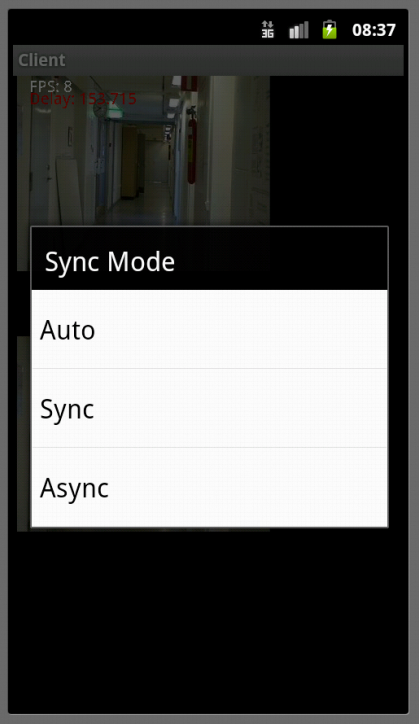
\includegraphics[width=0.75\textwidth]{../screenshots/androidSyncMode.png}
\caption{Screenshot of the Android client Sync Mode menue}
\end{figure}

\begin{figure}[hbp]
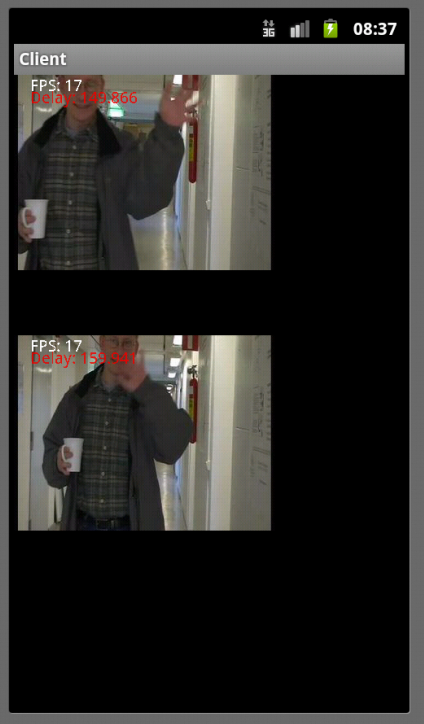
\includegraphics[width=0.75\textwidth]{../screenshots/androidSyncing.png}
\caption{Screenshot of the Android client syncing frames}
\end{figure}








\section{Server side}
The server side consist of two servers CameraServer and FakeCameraServer, where the former run against camera proxy servers and the latter is mostly for test, demo or debug purposes.



\subsection{CameraThread}
A camera server has a thread called CameraThread dedicated for fetching images from a proxy camera (or maybe from hardware - untested). The fetched images are put in the FrameBuffer mailbox of the SendThread associated with a connected client. The used cameras have capabilities to detect motion. This is used by the CameraThread if the current display mode is set to AUTO, then a motion detect will trigger a display mode MOVIE message to be put in the associated SendThreads CircularBuffer mailbox. To set the display mode to AUTO again a manual user reset is required. 

The user can switch to display mode MOVIE manually in addition to the automatic motion detect triggered switch.

In order to force the camera to periodically send images each fifth second there also exist a display mode IDLE.

\subsection{CameraMonitor}
Camera monitor exist to synchronize shared data for the camera server. In this case the shared data is only the current display mode. This is an integer value and could be atomically changed anyway but keeping it in a monitor held the door open to add more functionality later.

The figure below shows a UML diagram of the Camera Server system. 

\subsection{Embedded Http Server}
Camera Server support the option to run a lightweight embedded http server. The http server is started in it’s own thread by specifying the flag -http <port> when starting the camera server. The http server send an image every time a http client requests one, so one could theoretically refresh the image 24 times per second and get a live-stream in a browser of your choosing. This also means that the camera can be accessed from unsupported platforms such as iPhone.

\begin{figure}[hbp]
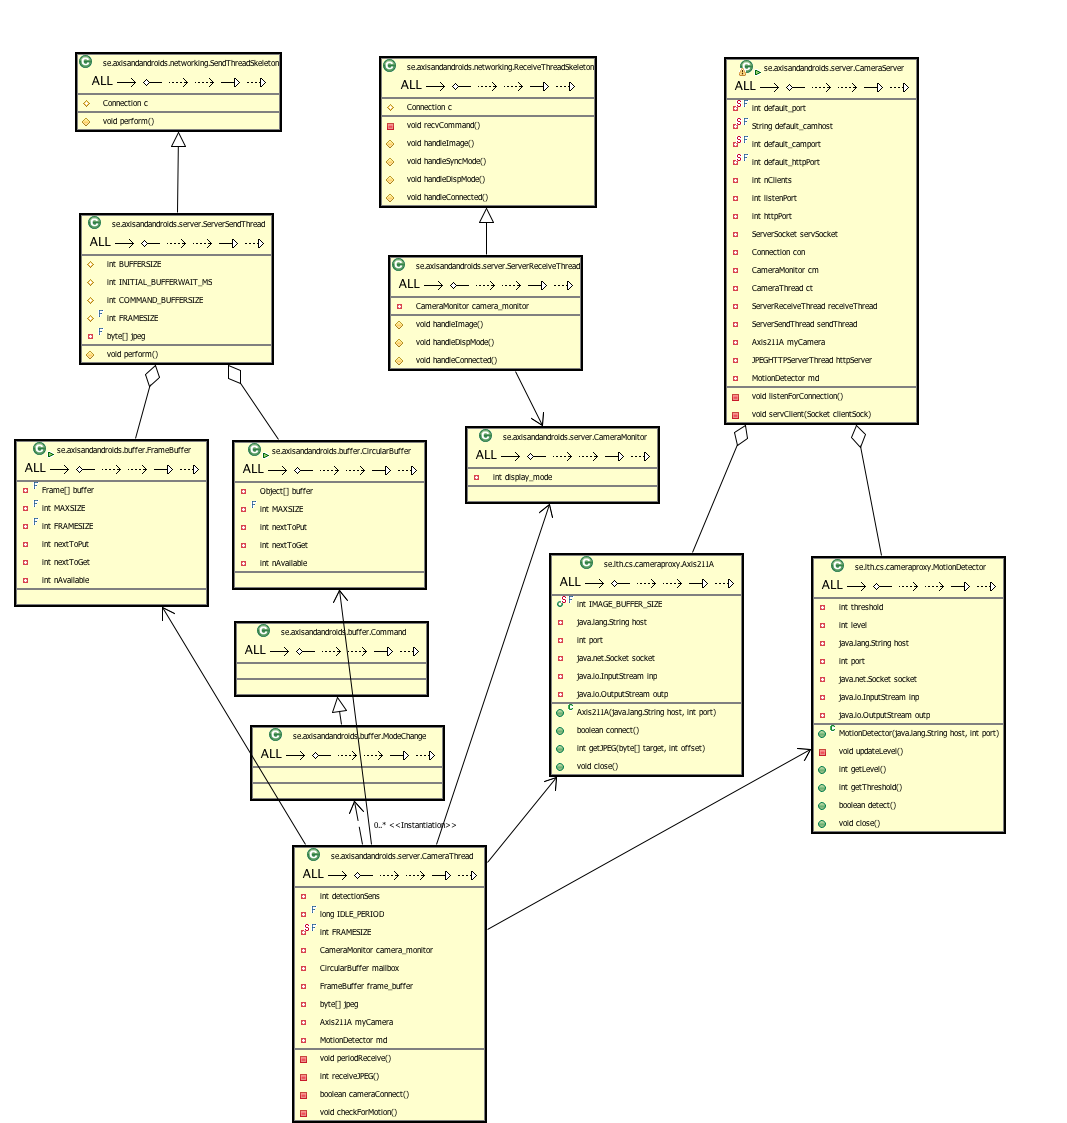
\includegraphics[width=0.75\textwidth]{../uml/server.png}
\caption{UML of the server side}
\end{figure}

The UML above shows how CameraMonitor recieves commands from both the RecieveThread and the CameraThread. This is because both the client and the camera itself can decide when to switch display modes. The CameraThread is also connected to the SendThread. This is because when a display mode occurs because of motion detection, it has to tell the client. The client then tells the other cameras to make the same switch.

\section{User guide}

\subsection{The fake camera server}
\begin{verbatim}
Start the server simply by typing 

SERVERNAME [options] [<PORT>]

Where <PORT> is the port you want the server to listen to. 
If the optional <PORT> is not used, it will by default listen to 
port 6000.

The different options are:

-help HELP!

\end{verbatim}

\subsection{The camera server}
\begin{verbatim}
Start the server simply by typing:

SERVERNAME [options] [optional: <PORT>]

Where <PORT> is the port you want the server to listen to. 
If the optional <PORT> is not used, it will by default listen 
to port 6000.

The different options are:

-camera <HOST> <PORT>  This option connects to a camera at the 
specified host
 and port. If this option isn't used the server will connect to 
 “argus-8.student.lth.se” at port 4321.

-http <PORT> 		This option starts the simple http server, listening 
at the specified port.

-help 				This option shows the help. It will guide you through the 
darkness that is AxisAndAndroids.
\end{verbatim}

\subsection{The client}
\begin{verbatim}
The client supports the use of multiple cameras. A dropbox is 
available to change the display modes. To start the client type:
CLIENTNAME [<CAMERA_HOST_NAME> <PORT>]

To connect to more cameras type in more host names and ports in 
the same manner. Eg. Client argus-1.student.lth.se 4321 
argus-2.student.lth.se 4321
If no hosts or ports are defined, it will use localhost and 
port 6000.
\end{verbatim}



\end{document}